\documentclass[hyperref={bookmarks=false},aspectratio=169]{beamer}
\usepackage{newtxtext}
\usepackage{amssymb}
\usepackage{amsthm}
\usepackage{bm}
\usepackage{amsmath}
\usepackage{color}
\usepackage{CJKutf8}
\usepackage{amsfonts}
\usepackage{mathrsfs}
\usepackage[justification=centering]{caption}
\usepackage{subcaption}
\usepackage{float}
\usepackage[linesnumbered,ruled,vlined]{algorithm2e}
\usepackage{cleveref}
\usepackage{booktabs}
\usepackage{seqsplit}
\usepackage{multirow}
\usepackage[utf8]{inputenc}
\usepackage[export]{adjustbox}
\usepackage{multirow,rotating}
\usepackage{hyperref}
\usepackage{tikz-cd}
\usepackage{array}
\usepackage{mathtools,nccmath}%
\usepackage{etoolbox, xparse} 
\usepackage[all]{xy}
\usepackage{tikz}
\usepackage[font={tiny}]{caption}
\usetikzlibrary{matrix,decorations.pathreplacing}


\newcommand*{\graybullet}{\textcolor{gray}{\textbullet}}
\newcommand*{\bluebullet}{\textcolor{blue}{\textbullet}}
\newcommand*{\redbullet}{\textcolor{red}{\textbullet}}


\NewDocumentCommand{\tens}{t_}
{%
	\IfBooleanTF{#1}
	{\tensop}
	{\otimes}%
}
\NewDocumentCommand{\tensop}{m}
{%
	\mathbin{\mathop{\otimes}\displaylimits_{#1}}%
}

% ---------------  Define theme and color scheme  -----------------
\usetheme[sidebarleft]{Gatech}  % 3 options: minimal, sidebarleft, sidebarright

%\setbeamertemplate{footline}[frame number]

% ------------  Information on the title page  --------------------
\title[]
{Your Title}

%\subtitle{{\small based on \hyperlink{https://journals.aps.org/prd/pdf/10.1103/PhysRevD.99.035001}{Phys. Rev. D 99, 035001}}}

\author[]
{{Your name}\\
\and Advisor}

\institute[Your Institute]
{
	 Your school\\
  Your institute
}

\date[]
{}	

% logo of sponser
\titlegraphic{\vspace{-1cm}

\includegraphics[height=1.5cm, valign=c]{Presentation/figures/NSFLogo.jpg}
\hfill

\includegraphics[height=1cm, valign=c]{Presentation/figures/DOElogo.jpg}
}

%------------------------------------------------------------
%The next block of commands puts the table of contents at the 
%beginning of each section and highlights the current section:

\AtBeginSection[]
{
  \begin{frame}
    \frametitle{Outline}
    \tableofcontents[currentsection,hideothersubsections]
  \end{frame}
}
%------------------------------------------------------------


\begin{document}

\frame{\titlepage}  % Creates title page

%---------   table of contents after title page  ------------
%\begin{frame}
%\frametitle{Outline}
%\tableofcontents
%\end{frame}
%---------------------------------------------------------

\section{Section 1}

%---------------------------------------------------------

\begin{frame}{Insert figures and texts}
\begin{columns}
\column{0.48\textwidth}
\vspace{-0.2cm}
\begin{figure}
    \centering
    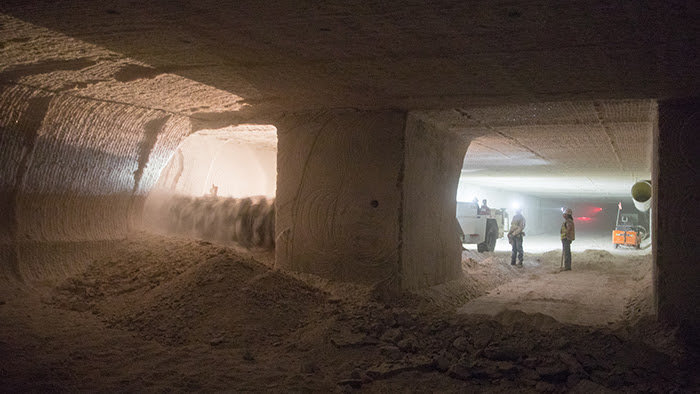
\includegraphics[width=0.8\textwidth]{Presentation/figures/SaltRockRepo.jpg}
    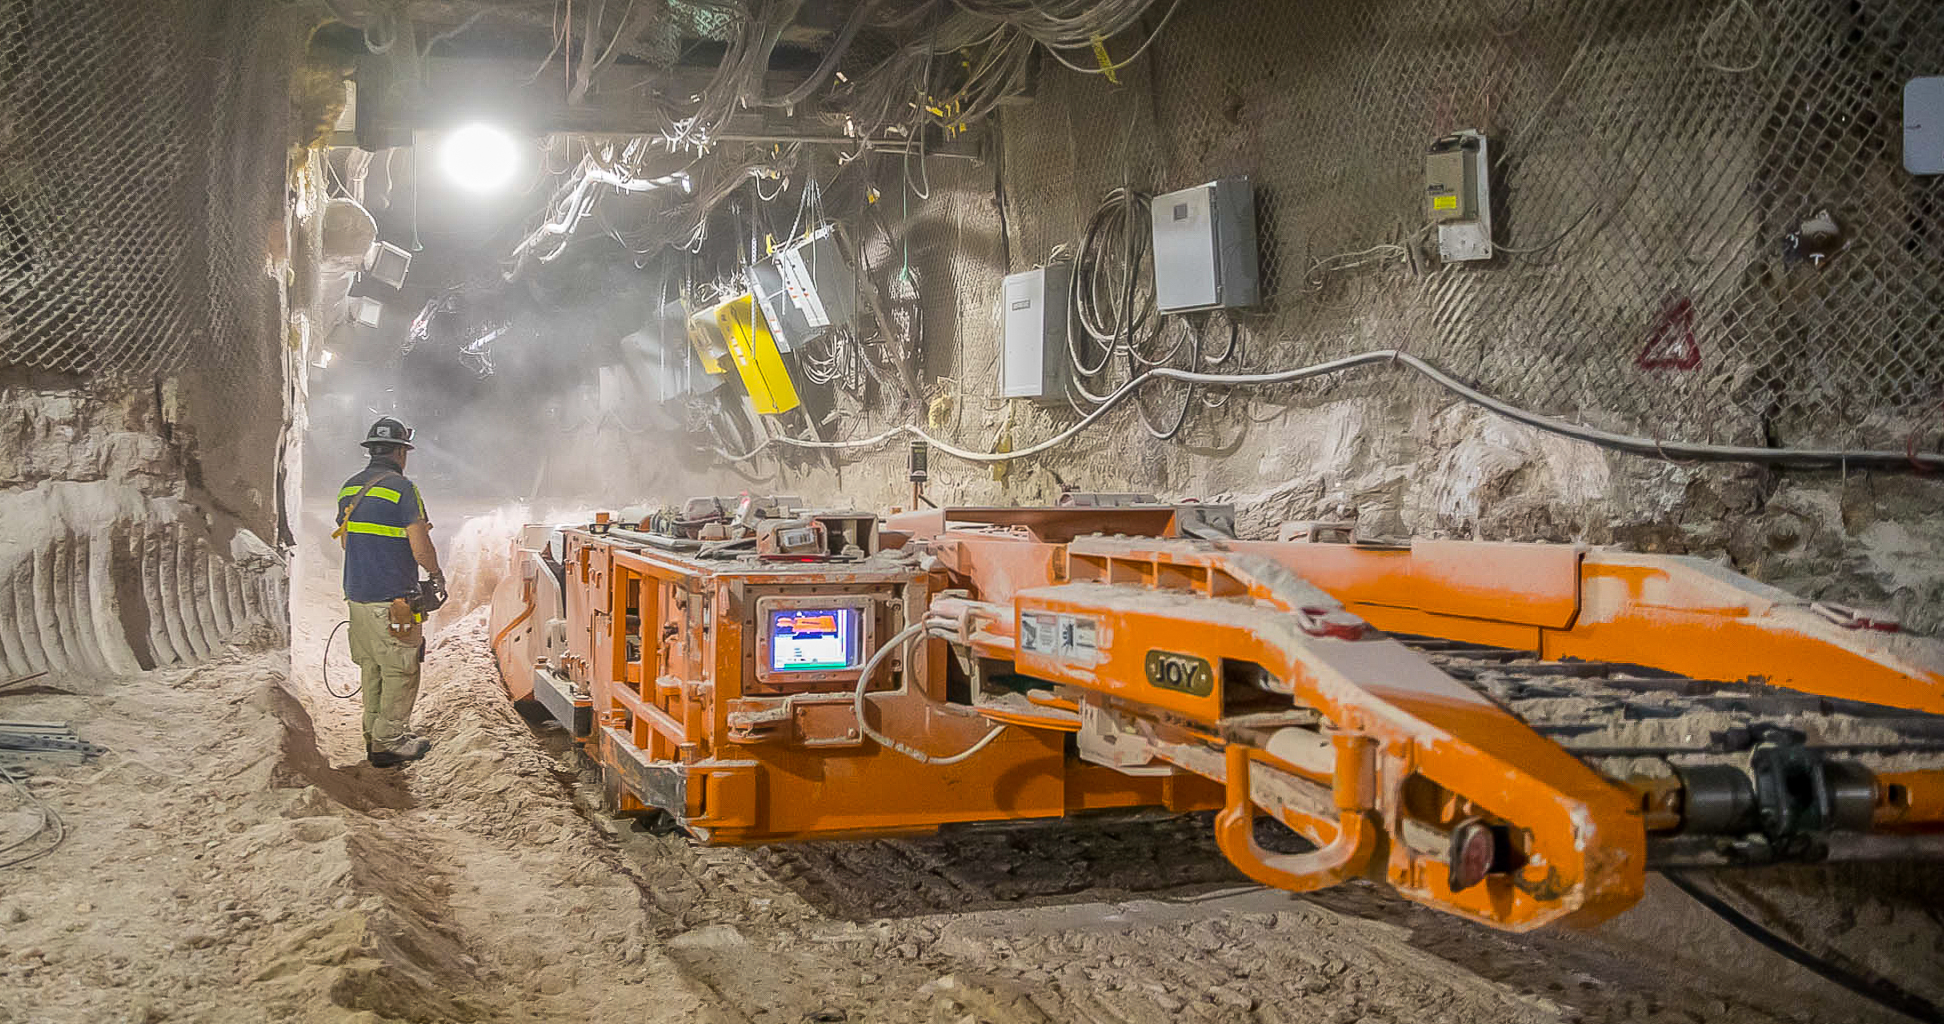
\includegraphics[width=0.8\textwidth]{Presentation/figures/WIPPsites.jpg}
    \caption{Waste Isolation Pilot Plant (WIPP) --- the nation's only deep geologic long-lived radioactive waste repository.}
\end{figure}
\quad
\column{0.48\textwidth}
Salt formation for \textcolor{myblue}{storage and disposal} of radioactive wastes:
\begin{enumerate}
   \item[$\blacksquare$] high thermal conductivity.

    \item[$\blacksquare$] low permeability.

    \item[$\blacksquare$] \textcolor{myred}{self-healing mechanism}.
    
    \item[$\blacksquare$] biologically inactivity (as compared with clay).
\end{enumerate}
\end{columns}
\end{frame}

%---------------------------------------------------------

\begin{frame}{Insert bullet points}
\begin{columns}
\column{0.48\textwidth}
\textcolor{myblue}{Problems to solve}:
\begin{enumerate}
    \item[$\ast$] Phenomenological model for the \textcolor{Gold}{multiphysical processes};
    
    \item[$\ast$] Lack of the \textcolor{Gold}{microscopic descriptions} $\Rightarrow$ difficult to capture certain behaviors, especially when they are coupled.
\end{enumerate}

\column{0.48\textwidth}
\textcolor{Navy}{Contributions}:
\begin{enumerate}
    \item[$\blacksquare$] Capture the physics of \textcolor{myred}{microscopic behaviors} and provide an explanatory framework of the \textcolor{myred}{macroscopic behaviors}; 
    
    \item[$\blacksquare$] Understand the \textcolor{myred}{mechanical and diffusion behaviors} in composites that exhibit complex \textcolor{myred}{microscopic deformation and mass exchange processes};
    
    \item[$\blacksquare$] Simulate \textcolor{myred}{boundary value problems} using the continuum model formulated at REV scale. 
\end{enumerate}
\end{columns}
\end{frame}

%--------------------------------------------------------

\section{Section 2}

%--------------------------------------------------------

\subsection{Subsection 1}

%--------------------------------------------------------

\subsection{Subsection 2}

%--------------------------------------------------------






   


\end{document}